\section{Đề số 28}

\begin{bt} 
   \hfill
   \begin{enumerate}[1.]
    \item \begin{enumerate}[a.]
        \item Thực hiện phép tính: $A=\left[\left(\frac{2}{193}-\frac{3}{386}\right) \cdot \frac{193}{17}+\frac{33}{34}\right]:\left[\left(\frac{7}{1008}+\frac{11}{2016}\right) \cdot \frac{1008}{25}+\frac{1007}{2016}\right]$
        \item Thực hiện phép tính: $B=\frac{1}{-77^2} \cdot 7^4(-11)^2 \cdot 77^5 \cdot\left(\frac{1}{7^2}\right)^2:\left(7^3 \cdot 11^6\right)$
    \end{enumerate}  
    \item Cho các số $a, b, c$ khác 0 thỏa mãn: $\frac{a-b+c}{2 b}=\frac{c-a+b}{2 a}=\frac{a-c+b}{2 c}$\\[5px]
    Tính giá trị biểu thức: $\mathrm{P}=\left(1+\frac{\mathrm{c}}{\mathrm{b}}\right) \cdot\left(1+\frac{\mathrm{b}}{\mathrm{a}}\right) \cdot\left(1+\frac{\mathrm{a}}{\mathrm{c}}\right)$
   \end{enumerate}
\loigiai{
    \begin{enumerate}[1.]
        \item \begin{enumerate}[a.]
              \item $A=\left[\left(\frac{2}{193}-\frac{3}{386}\right) \cdot \frac{193}{17}+\frac{33}{34}\right]:\left[\left(\frac{7}{1008}+\frac{11}{2016}\right) \cdot \frac{1008}{25}+\frac{1007}{2016}\right] \\[5px]
              A=\left[\frac{2}{17}-\frac{3}{34}+\frac{33}{34}\right]:\left[\left(\frac{7}{25}+\frac{11}{50}\right) \cdot+\frac{1007}{2016}\right] \\[5px]
              A=1:\left[\frac{1}{2}+\frac{1007}{2016}\right]$\\[5px] 
              $A=1:\left(\frac{2015}{2016}\right) \\[5px]
              A=\frac{2016}{2015}$\\[5px]
              Vậy $\quad \mathrm{A}=\frac{2016}{2015}$
              \item $B=\frac{1}{-77^2} \cdot 7^4(-11)^2 \cdot 77^5 \cdot\left(\frac{1}{7^2}\right)^2:\left(7^3 \cdot 11^6\right)$\\[5px]
              $B=\frac{1}{-7^2 \cdot 11^2} \cdot 7^4 \cdot 11^2 \cdot 7^5 \cdot 11^5 \cdot \frac{1}{7^4} \cdot \frac{1}{7^3 \cdot 11^6} \\[5px]
              B=-\frac{7^9 \cdot 11^7}{7^9 \cdot 11^8} \\[5px]
              B=-\frac{1}{11}$\\[5px]
              Vậy $B=-\frac{1}{11}$.
            \end{enumerate}
        \item Ta có: \\[5px] 
        $\mathrm{P}=\left(1+\frac{\mathrm{c}}{\mathrm{b}}\right)\left(1+\frac{\mathrm{b}}{\mathrm{a}}\right)\left(1+\frac{\mathrm{a}}{\mathrm{c}}\right)=\frac{\mathrm{b}+\mathrm{c}}{\mathrm{b}} \cdot \frac{\mathrm{a}+\mathrm{b}}{\mathrm{a}} \cdot \frac{\mathrm{c}+\mathrm{a}}{\mathrm{c}}\\[5px] 
        =\frac{\mathrm{b}+\mathrm{c}}{\mathrm{a}} \cdot \frac{\mathrm{a}+\mathrm{b}}{\mathrm{c}} \cdot \frac{\mathrm{c}+\mathrm{a}}{\mathrm{b}}$ với $\mathrm{a}, \mathrm{b}, \mathrm{c} \neq 0$\\[5px] 
        Khi $a+b+c=0 \Rightarrow\left\{\begin{array}{l}a+b=-c \\[5px] b+c=-a \\[5px] c+a=-b\end{array} \Rightarrow P=\frac{-a}{a} \cdot \frac{-c}{c} \cdot \frac{-b}{b}=-1\right.$\\[5px]
        Khi $a+b+c \neq 0$, áp dụng tính chất của dãy tỉ số bằng nhau ta có:\\[5px]
        $\frac{a-b+c}{2 b}=\frac{c-a+b}{2 a}=\frac{a-c+b}{2 c}=\frac{a-b+c+c-a+b+a-c+b}{2(c+a+b)}=\frac{1}{2} \\[5px]
        \Rightarrow \frac{a+c}{2 b}=\frac{c+b}{2 a}=\frac{a+b}{2 c}=1 \Rightarrow \frac{a+c}{b}=\frac{c+b}{a}=\frac{a+b}{c}=2 \\[5px]
        \Rightarrow P=8$\\[5px]
        Với $a, b, c \neq 0$ thì $P=-1$ khi $a+b+c=0 ; P=8$ khi $a+b+c \neq 0$
    \end{enumerate}
    
}
\end{bt}

\begin{bt}
    \hfill
	\begin{enumerate}[a.]
        \item Tìm $x$ biết: $\frac{2}{|x-2|+2}=\frac{3}{|6-3 x|+1}$
        \item Tìm hình chữ nhật có kích thước các cạnh là số nguyên sao cho số đo diện tích bằng số đo chu vi.
        \item Tìm các số nguyên dương x; y; z thỏa mãn:
        $$
        (x-y)^3+(y-z)^2+2015 \cdot|x-z|=2017
        $$
    \end{enumerate}
	\loigiai{
        \begin{enumerate}
            \item $\text {Tìm } x \text { biết : } \frac{2}{|x-2|+2}=\frac{3}{|6-3 x|+1} \\[5px]
            \frac{2}{|x-2|+2}=\frac{3}{3|x-2|+1} \Leftrightarrow 6|x-2|+2=3|x-2|+6 \Leftrightarrow 3|x-2|=4 \\[5px]
            \Leftrightarrow|x-2|=\frac{4}{3} \Leftrightarrow\left[\begin{array} { l } 
            { x - 2 = \frac { 4 } { 3 } } \\[5px]
            { x - 2 = - \frac { 4 } { 3 } }
            \end{array} \left[\begin{array}{l}
            x=\frac{10}{3} \\[5px]
            x=\frac{2}{3}
            \end{array}\right.\right.$\\[5px] 
            Vậy $x \in\left\{\frac{10}{3} ; \frac{2}{3}\right\}$
            \item Gọi kích thước hình chữ nhật cần tìm là $x, y$ (đơn vị độ dài )\\[5px]
            $\left(x, y \in N^* ; x \geq y\right)$\\[5px]
            Ta có diện tích và chu vi hình chữ nhật lần lượt là : $x . y$ và $2(x+y)$\\[5px]
            Theo bài ra ta có : $\mathrm{x} . \mathrm{y}=2(\mathrm{x}+\mathrm{y})$ với $\mathrm{x}, \mathrm{y} \in \mathrm{N}^* ; \mathrm{x} \geq \mathrm{y}$\\[5px]
            $\Leftrightarrow x y-2 x-2 y=0 \\[5px]
            \Leftrightarrow x(y-2)-2(y-2)=4 \\[5px]
            \Leftrightarrow(y-2)(x-2)=4$\\[5px]
            Với $\mathrm{x}, \mathrm{y} \in \mathrm{N}^*$ ta có $(\mathrm{y}-2) ;(\mathrm{x}-2) \in \mathrm{Z}$\\[5px]
            $\Rightarrow y-2 ; x-2 \in u^{\prime}(4)=\{ \pm 1 ; \pm 2 ; \pm 4\}$ nhưng vì $x-2 ; y-2>-2$ và $x \geq y$\\[5px]
            Ta có 2 trường hợp sau :\\[5px]
            $
            \left\{\begin{array} { l } 
            { x - 2 = 4 } \\[5px]
            { y - 2 = 1 }
            \end{array} \Leftrightarrow \left\{\begin{array} { l } 
            { x = 6 } \\[5px]
            { y = 3 }
            \end{array} \text { hoặc } \left\{\begin{array} { l } 
            { x - 2 = 2 } \\[5px]
            { y - 2 = 2 }
            \end{array} \Leftrightarrow \left\{\begin{array}{l}
            x=4 \\[5px]
            y=4
            \end{array}\right.\right.\right.\right.
            $\\[5px]
            Có hai hình chữ nhật thỏa mãn bài toán :\\[5px]
            Hình chữ nhật có kích thước 6 và 3 ; 4 và 4 .
            \item  Các bạn tự chứng minh: $(x-y)^3-(x-y)$ chia hết cho 2\\[5px]
            $(y-z)^2-(y-z)$ chia hết cho 2\\[5px]
            $|z-x|-(z-x)$ chia hết cho 2\\[5px]
            Do đó:\\[5px]
            $(x-y)^3+(y-z)^2+2015|x-z|= \\[5px]
            (x-y)^3-(x-y)+(y-z)^2-(y-z)+|z-x|-(z-x)+2014|z-x|$
            chia hết cho 2\\[5px]
            Mà 2017 không chia hết cho 2 nên không tồn tại các số nguyên dương x; y; z thỏa mãn đề bài.
        \end{enumerate}
    } 
\end{bt}

\begin{bt}
    Cho hàm số: $\mathrm{y}=\mathrm{f}(\mathrm{x})=\mathrm{x}+\frac{3}{2}|\mathrm{x}|(1)$
    \begin{enumerate}[a.]
        \item Vẽ đồ thị hàm số (1).
        \item Gọi $E$ và $F$ là hai điểm thuộc đồ thị hàm số (1) có hoành độ lần lượt là (-4) và $\frac{4}{5}$, xác định tọa độ hai điểm $\mathrm{E}, \mathrm{F}$. Tìm trên trục tung điểm $\mathrm{M}$ để $EM+MF$ nhỏ nhất.
    \end{enumerate}
	\loigiai{
        \begin{enumerate}
            \item Vẽ đồ thị hàm số $\mathrm{y}=\mathrm{f}(\mathrm{x})=\mathrm{x}+\frac{3}{2}|\mathrm{x}|$ (1)\\[5px]
            Từ hàm số (1) , ta có : $\quad \mathrm{y}=\frac{5}{2} \mathrm{x}$ với $x \geq 0$\\[5px]
            $y=\frac{-1}{2} x \text { với } x<0$\\[5px]
            Cho $\mathrm{x}=2 \Rightarrow \mathrm{y}=5$, ta có điểm $\mathrm{A}(2 ; 5)$ thuộc đồ thị hàm số(1)\\[5px] 
            Cho $\mathrm{x}=-2 \Rightarrow \mathrm{y}=1$, ta có điểm $\mathrm{B}(-2$;1) thuộc đồ thị hàm số (1) Đồ thị hàm số (1) là hai tia OAvà $O B$\\[5px] 
            $$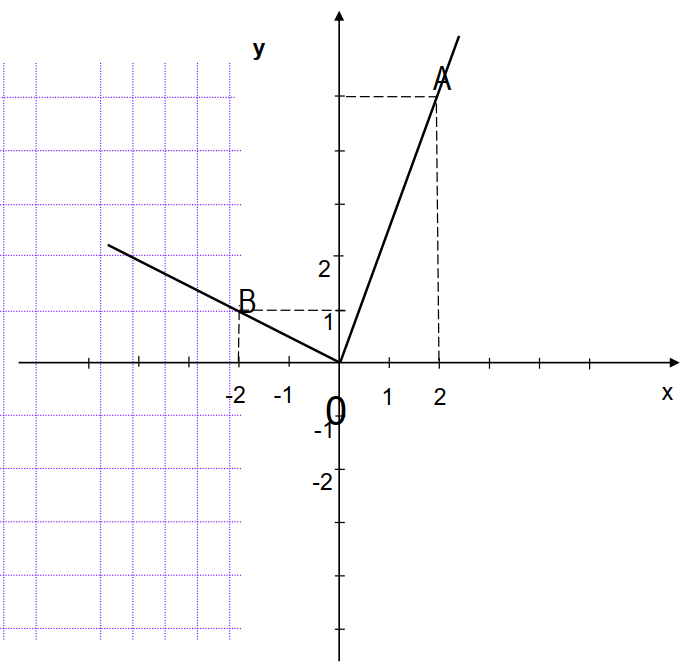
\includegraphics[width=0.4\textwidth]{28-3-lg.png}$$
            \item Từ hàm số (1) , ta có $\mathrm{y}=\frac{5}{2} \mathrm{x}$ với $x \geq 0$\\[5px]
            $y=\frac{-1}{2} x \text { với } x<0$\\[5px]
            Điểm E thuộc đồ thị hàm số (1) có hoành độ $\mathrm{x}=-4<0$\\[5px] 
            nên tung độ điểm $E$ là $\mathrm{y}=\frac{-1}{2}(-4)=2 \Rightarrow E(-4 ; 2)$\\[5px] 
            Điểm $\mathrm{F}$ thuộc đồ thị hàm số (1) có hoành độ $\mathrm{x}=\frac{4}{5}>0$\\[5px] 
            nên tung độ điểm $\mathrm{F}$ là $\mathrm{y}=\frac{5}{2} \cdot \frac{4}{5}=2 \Rightarrow \mathrm{F}(1 ; 2)\\[5px] 
            $ Điểm $M$ thuộc trục tung nên hoành độ điểm $M$ là $x=0$\\[5px] 
            Ta có $\mathrm{E}, \mathrm{F}$ thuộc đường thẳng $\mathrm{y}=2$\\[5px] 
            Để $\mathrm{EM}+\mathrm{FM}$ nhỏ nhất khi $\mathrm{M}$ nằm giữa $\mathrm{E}$ và $\mathrm{F}$\\[5px]
            nên $M$ thuộc đường thẳng $y=2$, nên tung độ $M$ là $y=2$\\[5px] 
            Vậy điểm M (0;2)
        \end{enumerate}
    }
\end{bt}

\begin{bt}
    \hfill
    \begin{enumerate}[1.]
        \item Cho tam giác $A B C$ nhọn; vẽ về phía ngoài tam giác $A B C$ các tam giác vuông cân tại $\mathrm{A}$ là tam giác $\mathrm{ABD}$ và tam giác $\mathrm{ACE}$.
        \begin{enumerate}[a.]
            \item Chứng minh $\mathrm{DC}=\mathrm{BE}$ và $\mathrm{DC} \perp \mathrm{BE}$.
            \item Gọi $\mathrm{H}$ là chân đường vuông góc kẻ từ $\mathrm{A}$ đến $\mathrm{ED}$ và $\mathrm{M}$ là trung điểm của đoạn thẳng $\mathrm{BC}$. Chứng minh $\mathrm{A}, \mathrm{M}, \mathrm{H}$ thẳng hàng .
        \end{enumerate}
        \item Cho tam giác $\mathrm{ABC}$ vuông tại $\mathrm{A}$ có $\mathrm{AB}=3 \mathrm{~cm} ; \mathrm{AC}=4 \mathrm{~cm}$. Điểm $I$ nằm trong tam giác và cách đều ba cạnh của tam giác $\mathrm{ABC}$. Gọi $\mathrm{M}$ là chân đường vuông góc kẻ từ điểm $I$ đến $BC$. Tính $MB$.
    \end{enumerate}
	\loigiai{
        \begin{enumerate}[1.]
            \item $$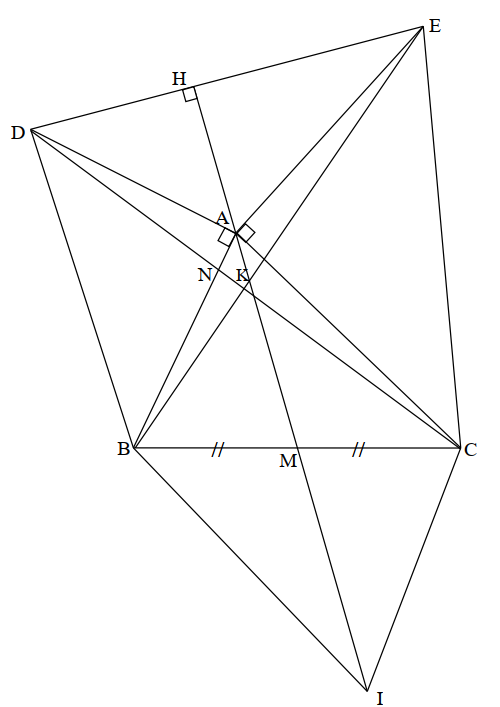
\includegraphics[width=0.45\textwidth]{28-4-lg.png}$$
            \begin{enumerate}[a.]
                \item Chứng minh $\mathrm{DC}=\mathrm{BE}$\\[5px]
                Ta có $\angle \mathrm{DAC}=\angle \mathrm{DAB}+\angle \mathrm{BAC}=90^{\circ}+\angle \mathrm{BAC}$ tương tự $\angle \mathrm{BAE}=90^{\circ}+\angle \mathrm{BAC}$\\[5px]
                $\Rightarrow \angle \mathrm{DAC}=\angle \mathrm{BAE}$\\[5px]
                Xét $\triangle \mathrm{DAC}$ và $\triangle \mathrm{BAE}$ có $\mathrm{AD}=\mathrm{AB}(\triangle \mathrm{ABD}$ vuông cân tại $\mathrm{A}$ )\\[5px]
                $\mathrm{AC}=\mathrm{AE}$ ( $\triangle \mathrm{AC}$ E vuông cân tại $\mathrm{A}$ )\\[5px]
                $\angle \mathrm{DAC}=\angle \mathrm{BAE}(\mathrm{cmt})$\\[5px]
                $\Rightarrow \Delta \mathrm{DAC}=\Delta \mathrm{BAE}(\mathrm{c}-\mathrm{g}-\mathrm{c})$\\[5px]
                $\Rightarrow \mathrm{DC}=\mathrm{BE} \quad$ ( định nghĩa tam giác bằng nhau)\\[5px]
                Chứng minh $\mathrm{DC} \perp \mathrm{BE}$\\[5px]
                Gọi $K, N$ lân lượt là giao điểm của $D C$ với $B E$ và $A B$\\[5px] 
                $\triangle \mathrm{AND}$ và $\triangle \mathrm{KNB}$ có $\quad \angle \mathrm{AND}=\angle \mathrm{KNB}($ đối đỉnh );
                $\angle \mathrm{ADN}=\angle \mathrm{KBN}(\Delta \mathrm{DAC}=\Delta \mathrm{BAE}) \\[5px]
                \Rightarrow \angle \mathrm{DAN}=\angle \mathrm{BKN} \text { định lí tổng } 3 \text { góc trong tam giác }) \\[5px]
                \text {Mà } \angle \mathrm{DAN}=90^{\circ}((\Delta \mathrm{ABD} \text { vuông cân tại } \mathrm{A}) \\[5px]
                \Rightarrow \angle \mathrm{BKN}=90^{\circ} \\[5px]
                \Rightarrow \mathrm{DC} \perp \mathrm{BE} \text { tại } \mathrm{K}$
                \item Chứng minh $\mathrm{A}, \mathrm{H}, \mathrm{M}$ thẳng hàng\\[5px]
                Trên tia đối của tia MA lấy điểm I sao cho MI=MA\\[5px]
                Chứng minh $\triangle \mathrm{AMB}=\Delta \mathrm{IMC}(\mathrm{cgc})$\\[5px]
                $\Rightarrow \mathrm{CI}=\mathrm{AB} \text { và } \mathrm{CI} / / \mathrm{AB}$\\[5px]
                Chứng minh $\angle \mathrm{ACI}=\angle \mathrm{DAE}$ ( cùng bù $\angle \mathrm{BAC})$\\[5px]
                Chứng minh $\Delta \mathrm{ACI}=\Delta \mathrm{EAD}(\mathrm{c}-\mathrm{g}-\mathrm{c})$\\[5px]
                $\Rightarrow \angle \mathrm{CAI}=\angle \mathrm{AED}$ mà $\angle \mathrm{AED}+\angle \mathrm{EAH}=90^{\circ}(\Delta \mathrm{AHE}$ vuông tại $\mathrm{H})$\\[5px]
                $\Rightarrow \angle \mathrm{CAI}+\angle \mathrm{EAH}=90^{\circ} \Rightarrow \angle \mathrm{MAH}=180^{\circ} \Rightarrow \mathrm{M}, \mathrm{A}, \mathrm{H}$ thẳng hàng
            \end{enumerate}
            \item $$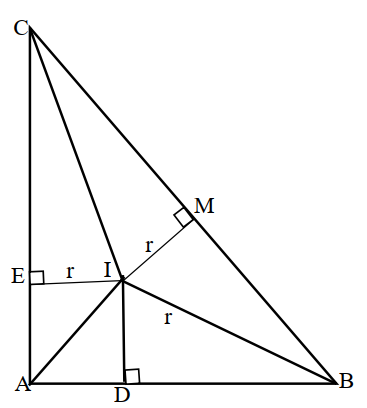
\includegraphics[width=0.45\textwidth]{28-4.2-lg.png}$$
            Vì điểm I nằm trong tam giác và cách đều 3 cạnh tam giác $\mathrm{ABC}$ nên I là giao điểm 3 đường phân giác trong tam giác $\mathrm{ABC}$\\[5px]
            Tam giác $\mathrm{ABC}$ vuông tại $\mathrm{A}$ nên $\mathrm{AB}^2+\mathrm{AC}^2=\mathrm{BC}^2$ ( định lý Pitago)\\[5px]
            Tính BC $=5 \mathrm{~cm}$\\[5px]
            Chứng minh $\Delta \mathrm{CEI}=\Delta \mathrm{CMI}$ (cạnh huyền- góc nhọn ) $\Rightarrow \mathrm{CE}=\mathrm{CM}$\\[5px]
            Tương tự $\mathrm{AE}=\mathrm{AD} ; \mathrm{BD}=\mathrm{BM}$\\[5px]
            Do đó:\\[5px] 
            $\mathrm{BM}=\frac{\mathrm{MB}+\mathrm{BD}}{2}=\frac{(\mathrm{BC}-\mathrm{MC})+(\mathrm{AB}-\mathrm{AD})}{2}=\frac{(\mathrm{BC}-\mathrm{CE})+(\mathrm{BA}-\mathrm{AE})}{2} \\[5px]
            =\frac{\mathrm{BC}+\mathrm{BA}-(\mathrm{AE}+\mathrm{EC})}{2}=\frac{\mathrm{BC}+\mathrm{BA}-\mathrm{AC}}{2} \\[5px]
            \Rightarrow B M=\frac{5+3-4}{2}=2(\mathrm{~cm})$
        \end{enumerate}
    }
\end{bt}

\begin{bt}
    Chứng minh rằng với mọi số tự nhiên $\mathrm{n} \geq 2$ thì tổng:
    $$
    \mathrm{S}=\frac{3}{4}+\frac{8}{9}+\frac{15}{16}+\ldots+\frac{\mathrm{n}^2-1}{\mathrm{n}^2} \text { không thể là một số nguyên. }
    $$
\loigiai{
    S có (n - 1) số hạng:\\[5px]
$S=\frac{3}{4}+\frac{8}{9}+\frac{15}{16}+\ldots+\frac{\mathrm{n}^2-1}{\mathrm{n}^2}=\left(1-\frac{1}{2^2}\right)+\left(1-\frac{1}{3^2}\right)+\left(1-\frac{1}{4^2}\right)+\ldots+\left(1-\frac{1}{\mathrm{n}^2}\right) \\[5px]
S=n-1-\left(\frac{1}{2^2}+\frac{1}{3^2}+\frac{1}{4^2}+\ldots+\frac{1}{\mathrm{n}^2}\right)<\mathrm{n}-1$(1)\\[5px]
Mặt khác $\frac{1}{2^2}+\frac{1}{3^2}+\frac{1}{4^2}+\ldots+\frac{1}{\mathrm{n}^2}<\frac{1}{1.2}+\frac{1}{2.3}+\frac{1}{3.4}+\ldots .+\frac{1}{(\mathrm{n}-1) \mathrm{n}}=1-\frac{1}{\mathrm{n}}$\\[5px]
$\mathrm{S}>\mathrm{n}-1-1+\frac{1}{\mathrm{n}}=\mathrm{n}-2+\frac{1}{\mathrm{n}}>\mathrm{n}-2$(2)\\[5px]
Từ (1) và (2) ta có $n-2<S<n-1$\\[5px]
Vậy $\mathrm{S}$ không có giá trị nguyên với mọi số tự nhiên $\mathrm{n} \geq 2$
}
\end{bt}


